\documentclass[xcolor=dvipsnames]{beamer}
\usepackage[utf8]{inputenc}
\usepackage[T1]{fontenc}
\usepackage{lmodern}
\usepackage{xcolor}
\usepackage{color}
\usepackage{enumitem}
\usepackage{tikz}

\setlist[itemize,1]{label=\textbullet}
\setlist[itemize,2]{label=$-$}

%\usebackgroundtemplate{\includegraphics[width=\paperwidth,height=\paperheight]{images/forma4.png}}
\setbeamercolor{frametitle}{bg=Gray, fg=white}
\setbeamercolor{normal text}{fg=black}

\setbeamercolor{title}{fg=white}
\setbeamercolor{titlelike}{fg=white}
\setbeamercolor{structure}{bg=Gray, fg=black}
\useoutertheme{shadow}
%\useinnertheme{rounded}

\beamertemplatenavigationsymbolsempty

\setbeamertemplate{footline}[frame number] 
\setbeamertemplate{headline}{}

%\renewcommand*{\bibfont}{\footnotesize}
\bibliographystyle{plain}

\title{Ground-Truth-Renderer für Partikelbasierte Daten}
\author{Josef Schulz}
\institute{Technische Universität Dresden}

\begin{document}

\begin{frame}
	\maketitle
	\nocite*{}
	\thispagestyle{empty}
\end{frame}

\begin{frame}
	\frametitle{Aufgabenstellung}
	
	Ziel der Arbeit:	
	
	\vspace*{0.4cm}
	
	\begin{itemize}
		\setlength{\itemsep}{8pt}
		
		\item Entwicklung eines CPU-Renderers für Partikeldaten
		\item basierend auf dem Emissions- und Absorptionsmodell
		\item Unterstützung von beliebig vielen Punkt und Richtungslichtquellen
		\item Beschränkung auf Kugelglyphen
	\end{itemize}
	
	\vspace*{0.2cm}
	
	\begin{itemize}
		\item Genauigkeit wird Geschwindigkeit übergeordnet
		\item liefert Ground-Truth-Bilder
	\end{itemize}
\end{frame}

\begin{frame}
	\frametitle{Wissenschaftliche Herausforderungen}
	
	Kugelglyphen werden mit Methoden der Volumendarstellung visualisiert: 
	
	\begin{itemize}
		\setlength{\itemsep}{8pt}
	
		\item physikalische Plausibilität des Modells
		\item weitestgehend Analytische Lösung
		\item kompakte und geschlossene Gleichung
		\item Genauigkeit wird Geschwindigkeit übergeordnet
		\item Ground-Truth
	\end{itemize}
	
	\vspace*{0.4cm}
	
	Unterstützte Effekte:
	
	\begin{itemize}
		\item Transparenz
		\item globaler Schattenwurf
	\end{itemize}
\end{frame}

\begin{frame}
	\frametitle{Gliederung}
	\tableofcontents
\end{frame}

\section{\textbullet \hspace{0.2cm} Grundlagen}
\begin{frame}
	\frametitle{Was ist Partikel}
	
	Ein Partikel ist ein: \\
	\vspace{0.2cm}
	
	\begin{itemize}
		\item[-] beliebiges geometrisches Objekt
		\item[-] es wird durch eine Menge von Attributen beschrieben
		\item[-] die Position ist ein obligatorisch Attribut
	\end{itemize}

	\vspace{0.5cm}
	Parametrisierung eines kugelförmigen Partikels:
	
	\begin{columns}
		\begin{column}{3cm}
			\begin{figure}
				\def\svgwidth{3cm}
				\input{images/exPartikel.pdf_tex}
			\end{figure}
		\end{column}
		\begin{column}{7cm}
			\begin{itemize}
				\setlength{\itemsep}{8pt}
				\item \makebox[1cm]{$M$\hfill} - Position
				\item \makebox[1cm]{$r$\hfill} - Radius
				\item \makebox[1cm]{$I_C$\hfill} - Farbe
				\item \makebox[1cm]{$\Theta_{MAX}$\hfill} - maximaler Opazitätswert
			\end{itemize}
		\end{column}
	\end{columns}
	
	%\vspace{0.5cm}
	
\end{frame}

\begin{frame}
	\frametitle{Partikelvisualisierung}
	
	Visualisierung mit Methoden der direkten Volumendarstellung \\
	\vspace{0.5cm}
	Interpretation der Partikel als Gas gefüllte Kugeln
	\vspace{0.5cm}
	\begin{itemize}
		\setlength{\itemsep}{8pt}
		\item Transparenzeffekte
		\item Kugelform wird erhalten
		\item globale Schatten aufgrund von Lichtabschwächung
	\end{itemize}
\end{frame}

\begin{frame}
	\frametitle{Grundlegenste Arbeiten}
	
	\begin{itemize}
		\setlength{\itemsep}{20pt}
		\item{Optical Models for Direct Volume Rendering} \\ 
		\textasciitilde Nelson Max 
		\cite{Max:1995:OMD:614258.614298}
		\begin{itemize}
			\item Definition des EA-Modells
			\item \textcolor{Gray}{Einfache Streuung}
			\item \textcolor{Gray}{Schatten}
			\item \textcolor{Gray}{Mehrfach Streuung}
		\end{itemize}
		
		\item{Visualization of Particle-based Data with Transparency and Ambient Occlusion} \\
		\textasciitilde Joachim Staib, Sebastian Grottel und Stefan Gumhold
		\cite{CGF34-3:151-160:2015}
		\begin{itemize}
			\item Analytische Lösung der Rendergleichung
			\item \textcolor{Gray}{Ambiente Verdeckung}
		\end{itemize}
	\end{itemize}
\end{frame}

\section{\textbullet \hspace{0.2cm} Rendergleichung}
\subsection{\textbullet \hspace{0.2cm} EA-Modell}
\begin{frame}
	\frametitle{Rendergleichung}
	
	Emissions- und Absorptionsmodell von Nelson Max \cite{Max:1995:OMD:614258.614298}:
	
	\begin{align}
		I = \textcolor{blue}{I_A} &+ \textcolor{PineGreen}{I_E} \\
		I = \textcolor{blue}{I_B \cdot T'(0, D)} &+ \textcolor{PineGreen}{\int\limits_{0}^{D} g(s) \cdot T'(s, D) ds}
	\end{align}
	
	\vspace{0.3cm}
	
	\begin{description}
		\item Abschwächung: $T'(t_n, t_f) = \exp(- \int\limits_{t_n}^{t_f} \textcolor{Purple}{\tau(t)} dt)$;
		\item \makebox[0.7cm]{\textcolor{Purple}{$\tau$} \hfill} wird als Transferfunktion bezeichnet
		\item \makebox[0.7cm]{\textcolor{blue}{$I_B$}\hfill} Hintergrundbeleuchtung
		\item \makebox[0.7cm]{\textcolor{PineGreen}{g(s)}\hfill} Quellterm
	\end{description}
	
\end{frame}

\subsection{\textbullet \hspace{0.2cm} einfaches EA-Modell}
\begin{frame}
	\frametitle{Einfaches EA-Modell}
	
	Emissions- und Absorptionsmodell nach \cite{CGF34-3:151-160:2015}:
	
	\begin{figure}
		\def\svgwidth{8cm}
		\input{images/standartAbsorption.pdf_tex}
	\end{figure}
	
	\begin{equation}
		I = \textcolor{blue}{I_B \cdot T'(t_n, t_f)} + \textcolor{PineGreen}{\int\limits_{t_n}^{t_f} \textcolor{Purple}{g(s)} \cdot T'(s, t_f) ds}
		\label{eq:EAM}
	\end{equation}
	
	\vspace{0.3cm}
	
	Der Quellterm wird auf $\textcolor{Purple}{g(s) = \lambda\kappa \cdot I_C}$ gesetzt und  die Transferfunktion als
	$\tau(t) = \sigma(\nu(t)) = \lambda\kappa$
	
\end{frame}

\begin{frame}
	\frametitle{Einfaches EA-Modell}
	
	\begin{equation}
		I = \textcolor{blue}{I_B \cdot T'(t_n, t_f)} + \textcolor{PineGreen}{\int\limits_{t_n}^{t_f} \textcolor{Purple}{g(s)} \cdot T'(s, t_f) ds}
	\end{equation}
	
	\begin{figure}
		\def\svgwidth{5cm}
		\input{images/standartAbsorption.pdf_tex}
	\end{figure}
	
	\begin{align}
		%\setlength{\jot}{30pt}
		T'(t_n, t_f) &= \exp(- \int\limits_{t_n}^{t_f} \tau(t) dt) = \exp(-\lambda\kappa \cdot (t_f - t_n)) \\
		\Theta(t_n, t_f) &= 1 - T'(t_n, t_f)
	\end{align}
	
	\begin{equation}
		I = \textcolor{blue}{I_B \cdot T'(t_n, t_f)} + \textcolor{PineGreen}{I_C \cdot \Theta(t_n, t_f)}
		\label{eq:LEEAM}
	\end{equation}
\end{frame}

\begin{frame}
	\frametitle{Bestimmung von $\Theta_{MAX}$}
	
	Bestimmung von $\Theta_{MAX}$ ($\lambda$ ist ein globaler Parameter):
	
	\begin{equation}
		\Theta(t_n, t_f) = 1 - \exp(- \lambda \textcolor{Purple}{\kappa} (t_f - t_n))
	\end{equation}
	
	Ersetzung der Parameter:
	
	\begin{itemize}
		\item \makebox[1.5cm]{$\Theta$		\hfill} = $\Theta_{MAX}$
		\item \makebox[1.5cm]{$t_f - t_n$	\hfill} = $2 \cdot r$
	\end{itemize}
	
	daraus folgt:
	
	\begin{equation}
		\kappa = - \frac{1}{\lambda \cdot 2r} \ln(1 - \Theta_{MAX})
	\end{equation}
	
\end{frame}

\subsection{\textbullet \hspace{0.2cm} erweitertes EA-Modell}
\begin{frame}
	\frametitle{Erweitertes EA-Modell - Lichtquellentypen}
	
	\begin{columns}
		\begin{column}{3cm}
		Punktlichtquelle
		\end{column}
		\begin{column}{5cm}
			\begin{figure}
				\def\svgwidth{5cm}
				\input{images/exStandartAbsorption.pdf_tex}
			\end{figure}
		\end{column}
	\end{columns}
	
	\begin{columns}
		\begin{column}{3cm}
		Richtungslichtquelle
		\end{column}
		\begin{column}{5cm}
			\begin{figure}
				\def\svgwidth{5cm}
				\input{images/exStandartAbsorptionDir.pdf_tex}
			\end{figure}
		\end{column}
	\end{columns}

\end{frame}

\begin{frame}
	\frametitle{Erweitertes EA-Modell}
	
	Voraussetzung ist wieder die Gleichung \ref{eq:EAM} und es wird eine Richtungslichtquelle angenommen:
	
	\begin{equation}
		I = \textcolor{blue}{I_B \cdot T'(t_n, t_f)} + \textcolor{PineGreen}{\int\limits_{t_n}^{t_f} \textcolor{Purple}{g(s)} \cdot T'(s, t_f) ds}
	\end{equation}
	
	\begin{figure}
		\def\svgwidth{5cm}
		\input{images/exStandartAbsorptionDir.pdf_tex}
	\end{figure}
	
	Die Lösung des einfachen EA-Modells \ref{eq:LEEAM} wird als Quellterm eingesetzt:
	
	\begin{equation}
		\textcolor{Purple}{g(s)} = I_L \cdot T'(0, \textcolor{Sepia}{l(s)}) + I_C \cdot \Theta(0, \textcolor{Sepia}{l(s)})
	\end{equation}
	
	\begin{description}
		\item $\textcolor{Sepia}{l(s)}$ entspricht der Länge der Sekundärstrahlen im Medium
	\end{description}
	
\end{frame}

\begin{frame}
	\frametitle{Analytische Lösung für das erweiterte EA-Modell}
	
	Bestimmung von $\textcolor{Sepia}{l(s)}$ mit Hilfe der quadratischen Lösungsformel führt zu:
	
	\begin{equation}
		F(x) = \int I \cdot \exp(ax + b + \sqrt{cx^2 + dx + e}) dx
		\label{eq:l}
	\end{equation}
	
	Gleichung \ref{eq:l} lässt sich nicht elementar integrieren!
\end{frame}

\begin{frame}
	\frametitle{Nummerische Approximation}
	
	Approximation durch Riemann-Summen:
	
	\begin{columns}
		\begin{column}{3cm}
			\begin{equation}
				\int\limits_{0}^{D} f(x) dx \approx \sum\limits_{i=1}^{n} f(x_i) \Delta x \nonumber
			\end{equation}
			
			\begin{description}
				\item mit $\Delta x = \frac{D}{n}$
			\end{description}
		\end{column}
		\begin{column}{5cm}
			\begin{figure}
				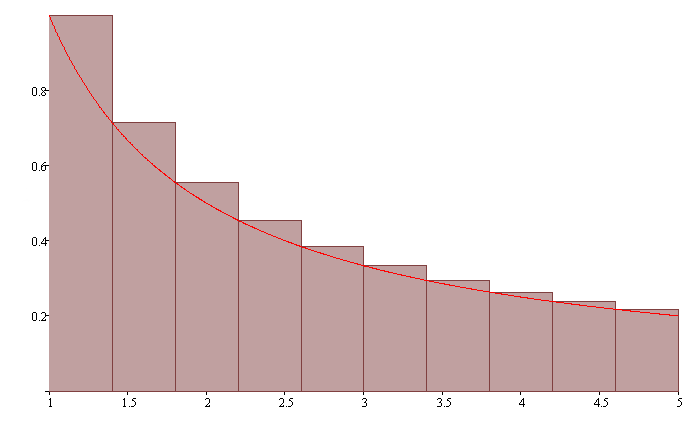
\includegraphics[width=5cm]{images/riemann.png}
			\end{figure}
		\end{column}
	\end{columns}
	
	\vspace{0.5cm}
	führt zur Endgültigen Rendergleichung:
	
	\begin{equation}
		I = \textcolor{blue}{I_B \cdot T'(t_n, t_f)} + \textcolor{PineGreen}{\sum\limits_{t_n}^{t_f} \textcolor{Purple}{g(s)} \cdot T'(s, t_f) \Delta s}
	\end{equation}
	
	\begin{equation}
		\textcolor{Purple}{g(s)} = \frac{1}{m} \left( \sum\limits_{i=1}^{m} I_{L_i} \cdot T'(0, \textcolor{Sepia}{l(s)}) + I_C \cdot \Theta(0, \textcolor{Sepia}{l(s)})\right)
	\end{equation}
	
\end{frame}

\begin{frame}
	\frametitle{Programmablauf}
	\begin{columns}
		\begin{column}{5cm}
			\begin{itemize}
				\item Kollisionstest
				\item Sortierung der Ergebnismenge
				\item für jede geschnittene Kugel:
				\begin{itemize}
					\item pro Sample ein Strahl zu jeder Lichtquelle
					\begin{itemize}
						\item[\textbullet] Kollisionstest, Sortierung
						\item[\textbullet] Abschwächung von $I_{L_i}$
					\end{itemize}
					\item erweitertes EA-Modell auswerten
				\end{itemize}
			\end{itemize}
		\end{column}
		\begin{column}{8cm}
			\begin{figure}
				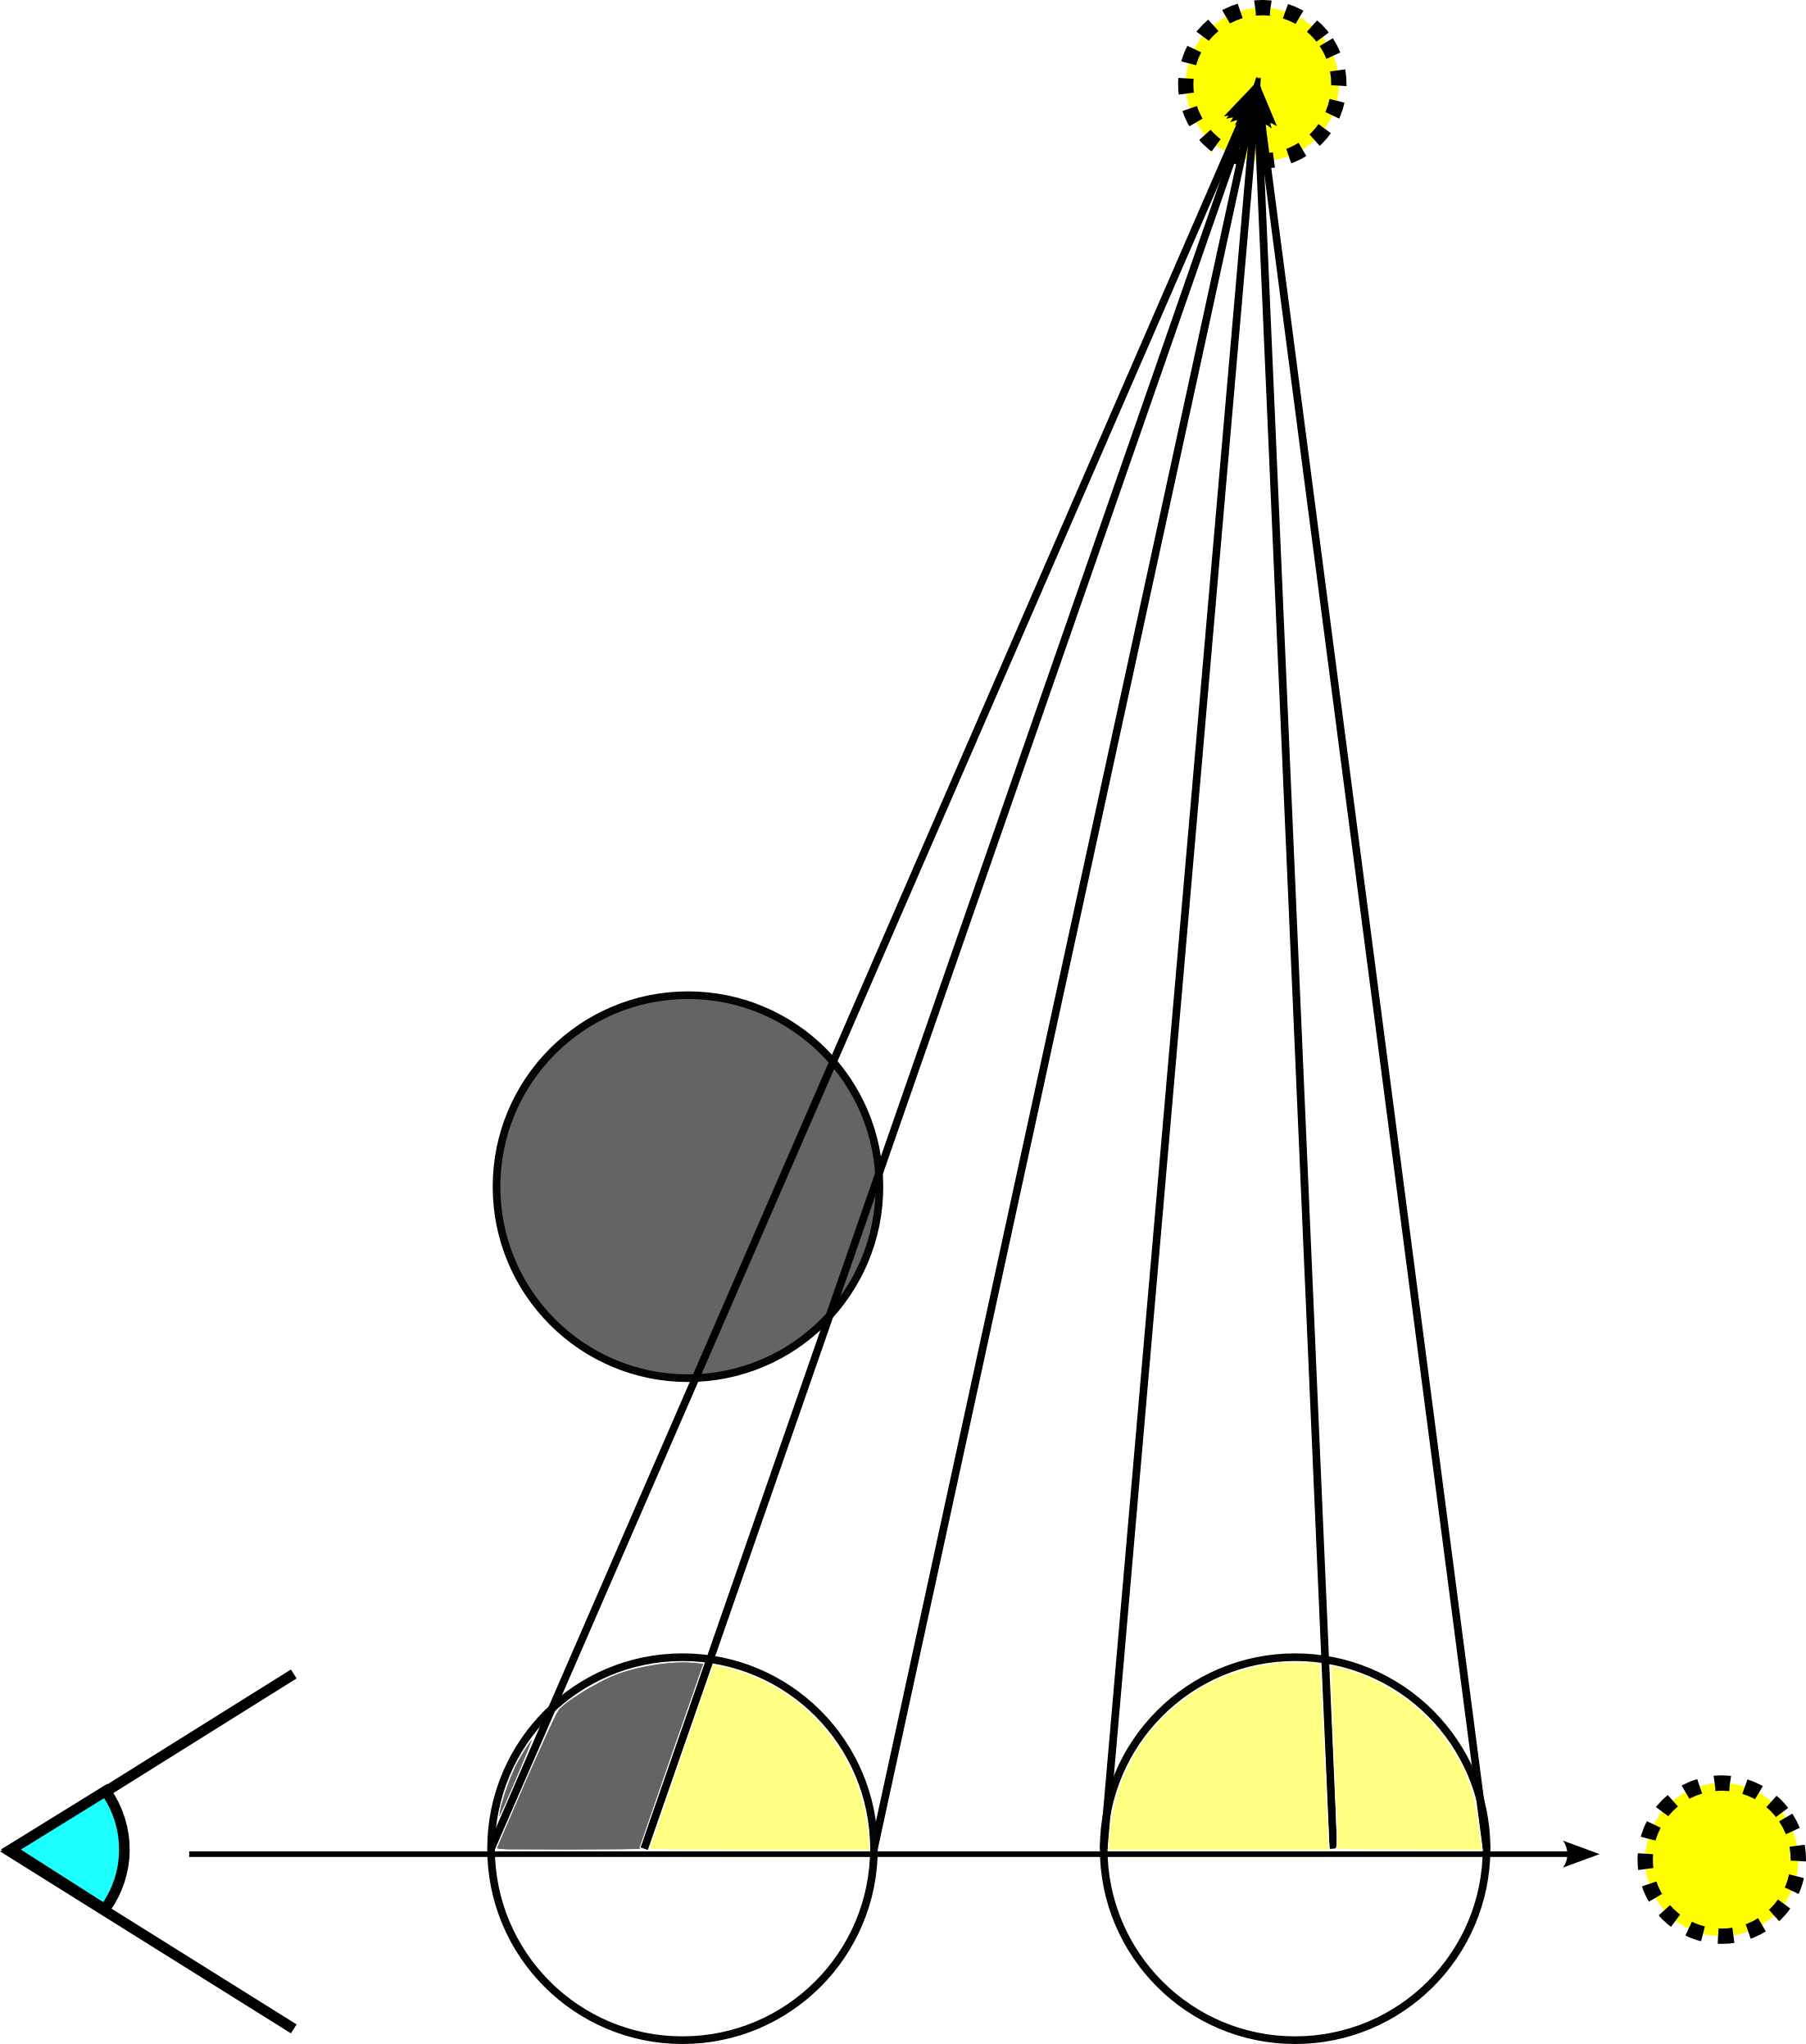
\includegraphics[width=6cm]{images/ablauf.png}
			\end{figure}
		\end{column}
	\end{columns}
	
\end{frame}

\section{\textbullet \hspace{0.2cm} Resultate}

{
	\usebackgroundtemplate{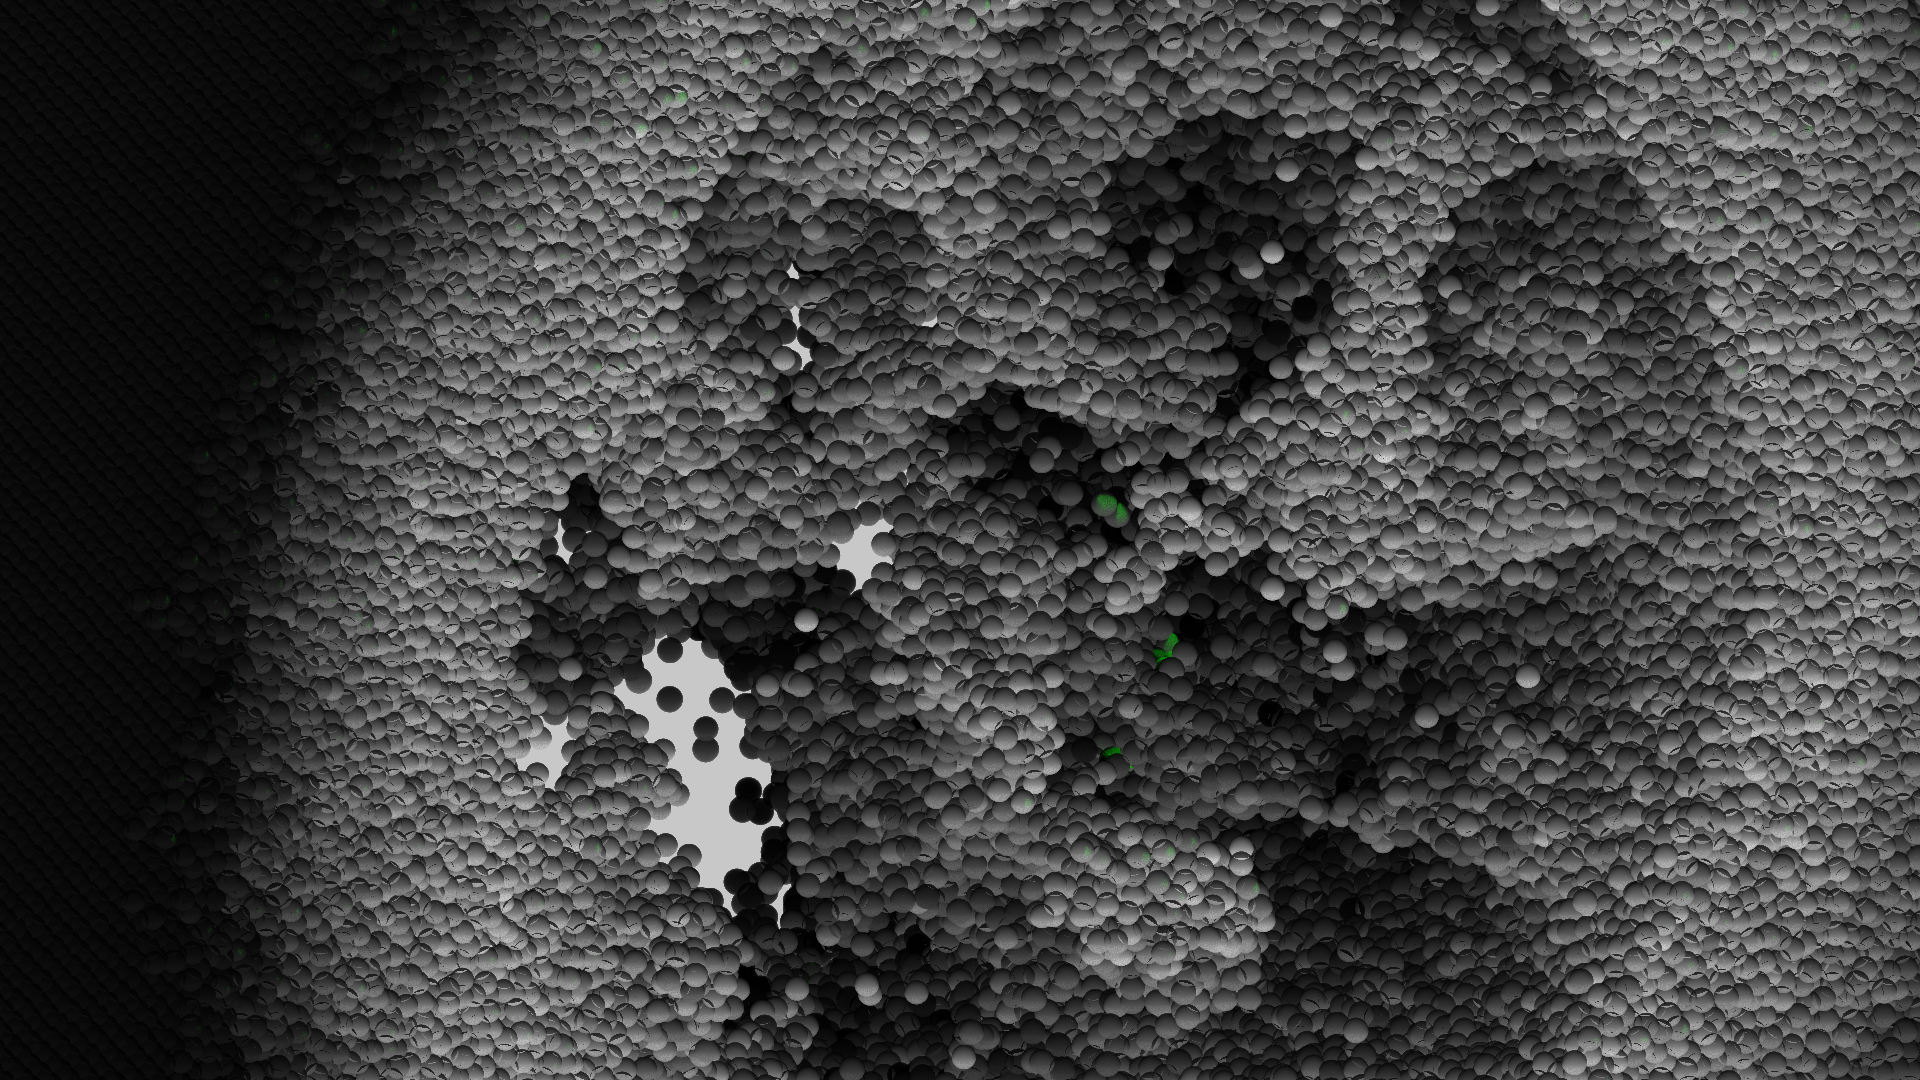
\includegraphics[height=\paperheight,width=\paperwidth]{images/imageLong.png}}
	\setbeamertemplate{navigation symbols}{}
	\begin{frame}[plain]
	\end{frame}
}

\begin{frame}
	\frametitle{Programmablauf mit Approximation}
	\begin{columns}
		\begin{column}{5cm}
			\begin{itemize}
				\item Programmablauf fast genau der gleiche
				\item Auswertung erweitertes EA-Modell für die vordersten $k$ Kugeln
			\end{itemize}
		\end{column}
		\begin{column}{8cm}
			\begin{figure}
				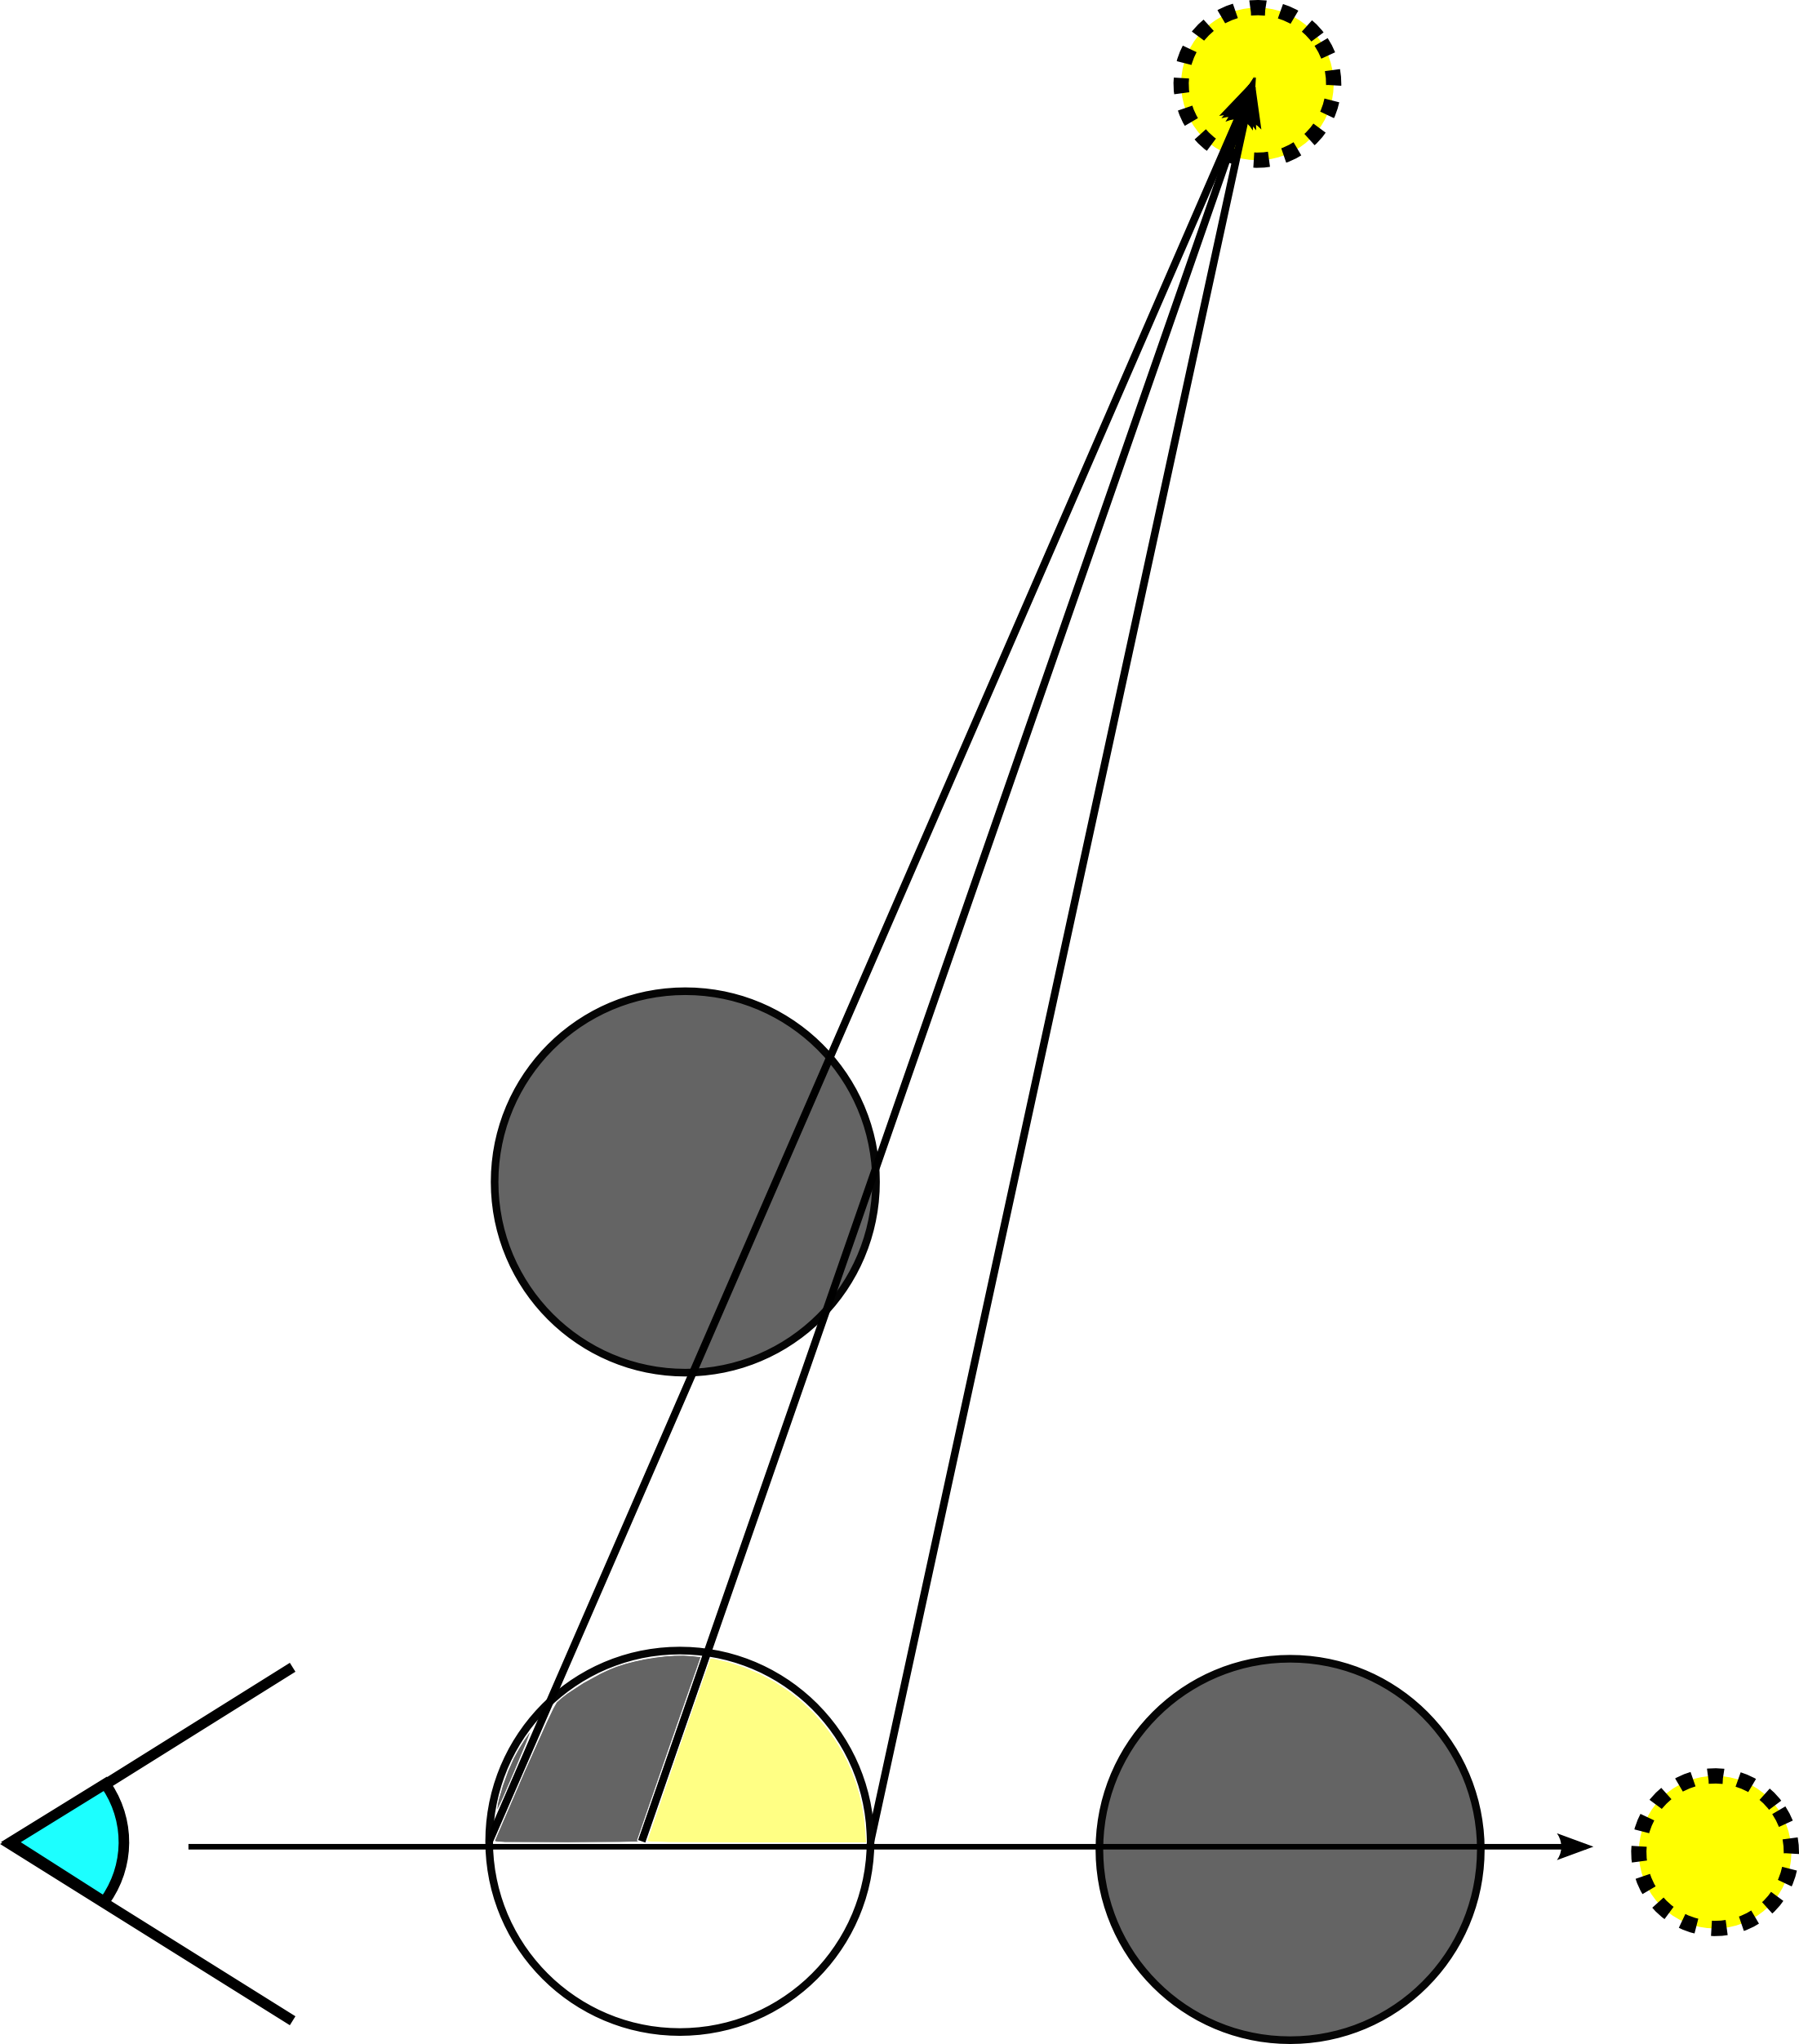
\includegraphics[width=6cm]{images/ablaufApprox.png}
			\end{figure}
		\end{column}
	\end{columns}
	
\end{frame}

\begin{frame}
	\frametitle{Abbildung der Renderzeiten}
	
	\begin{columns}
		\begin{column}{8cm}
			\begin{figure}
				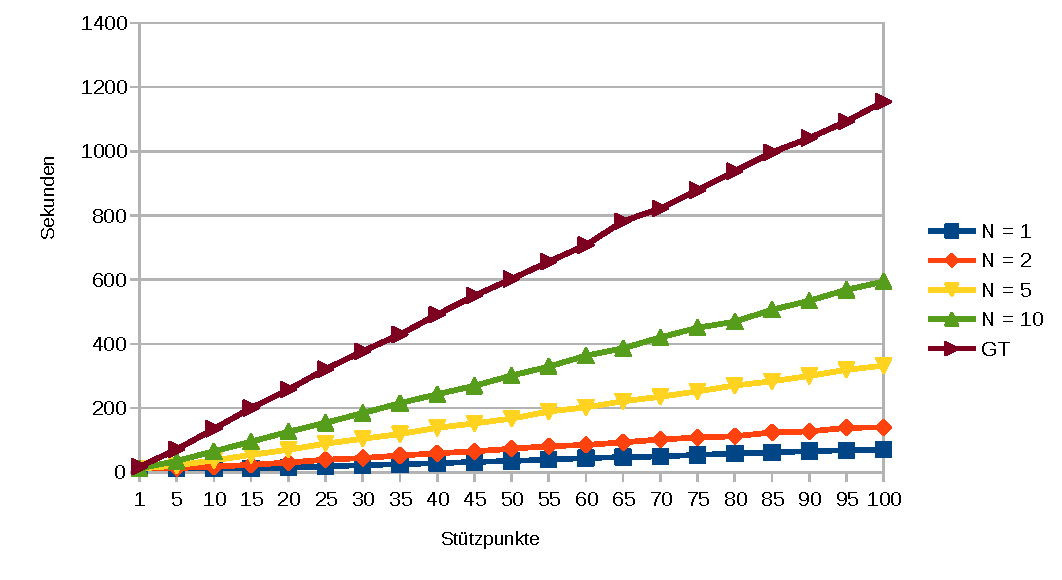
\includegraphics[width=8cm]{images/cool_random.pdf}
			\end{figure}
		\end{column}
		\begin{column}{5cm}
			\begin{table}[h]
				\centering
				\begin{tabular}{|c|c|}
					\hline
					$N$ & Mittelwert \\
					\hline
					1  & 77.1702\% \\
					2  & 91.8247\% \\ 
					5  & 99.9166\% \\
					10 & 99.9996\% \\
					\hline
				\end{tabular}
			\end{table}
		\end{column}
	\end{columns}
	\vspace{1cm}
	Unterschied, bereits nach 2 N weniger als 10 \% \footnote[1]{Genauigkeitsbestimmung mit SSIM \cite{Wang04imagequality}}
\end{frame}

{
	\usebackgroundtemplate{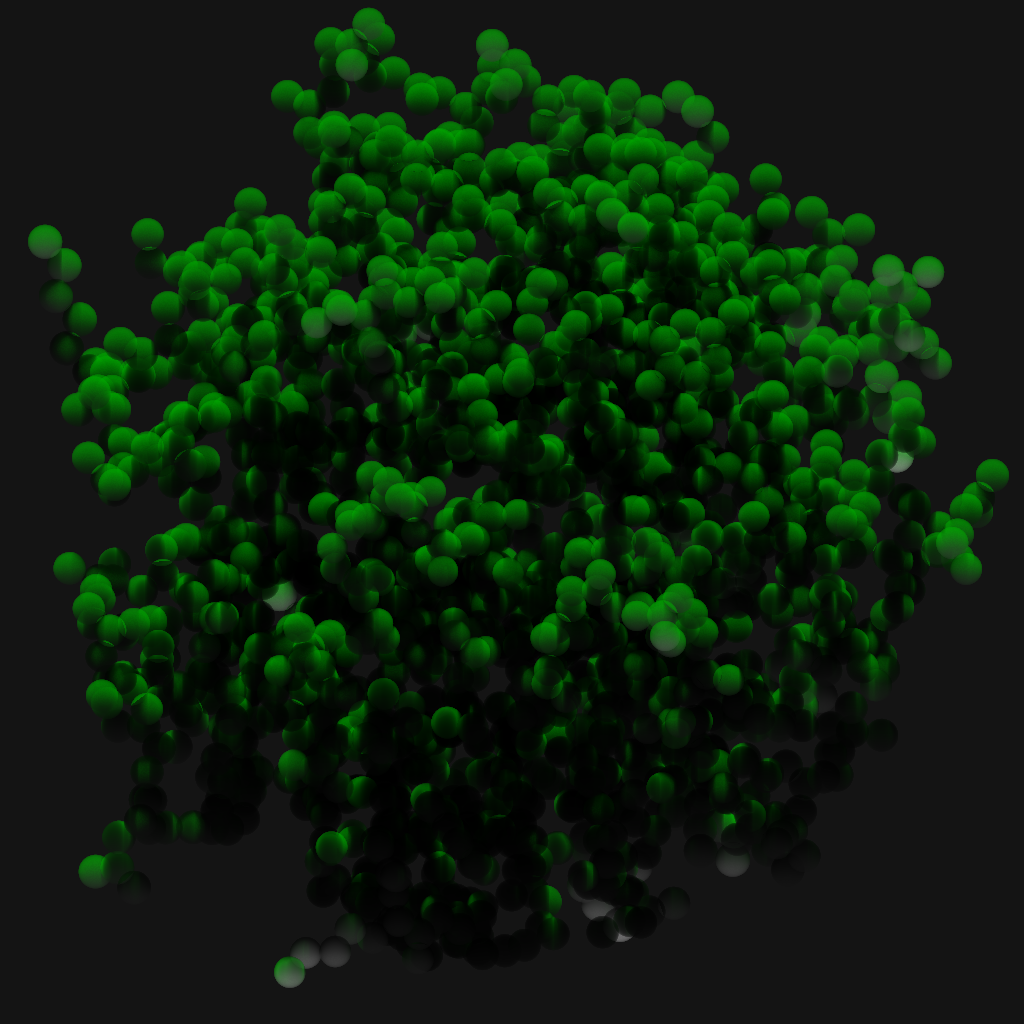
\includegraphics[height=\paperheight,width=\paperwidth]{images/shadowEEA.png}}
	\setbeamertemplate{navigation symbols}{}
	\begin{frame}[plain]
	\end{frame}
}

{
	\usebackgroundtemplate{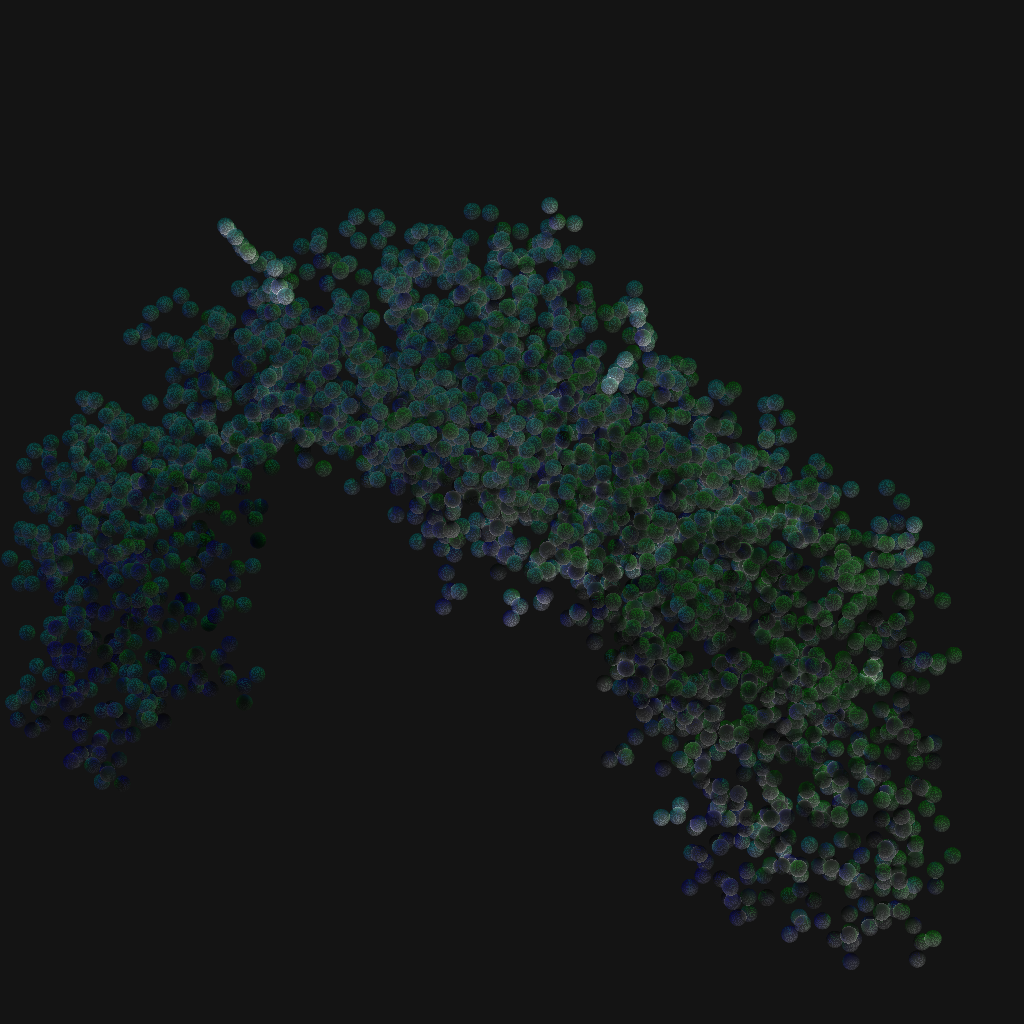
\includegraphics[height=\paperheight,width=\paperwidth]{images/512x512_samples_5_approx_1.png}}
	\setbeamertemplate{navigation symbols}{}
	\begin{frame}[plain]
	\end{frame}
}

\begin{frame}
	\frametitle{Transparenzprobleme}
	
	\begin{columns}
		\begin{column}{3cm}
			\begin{figure}
				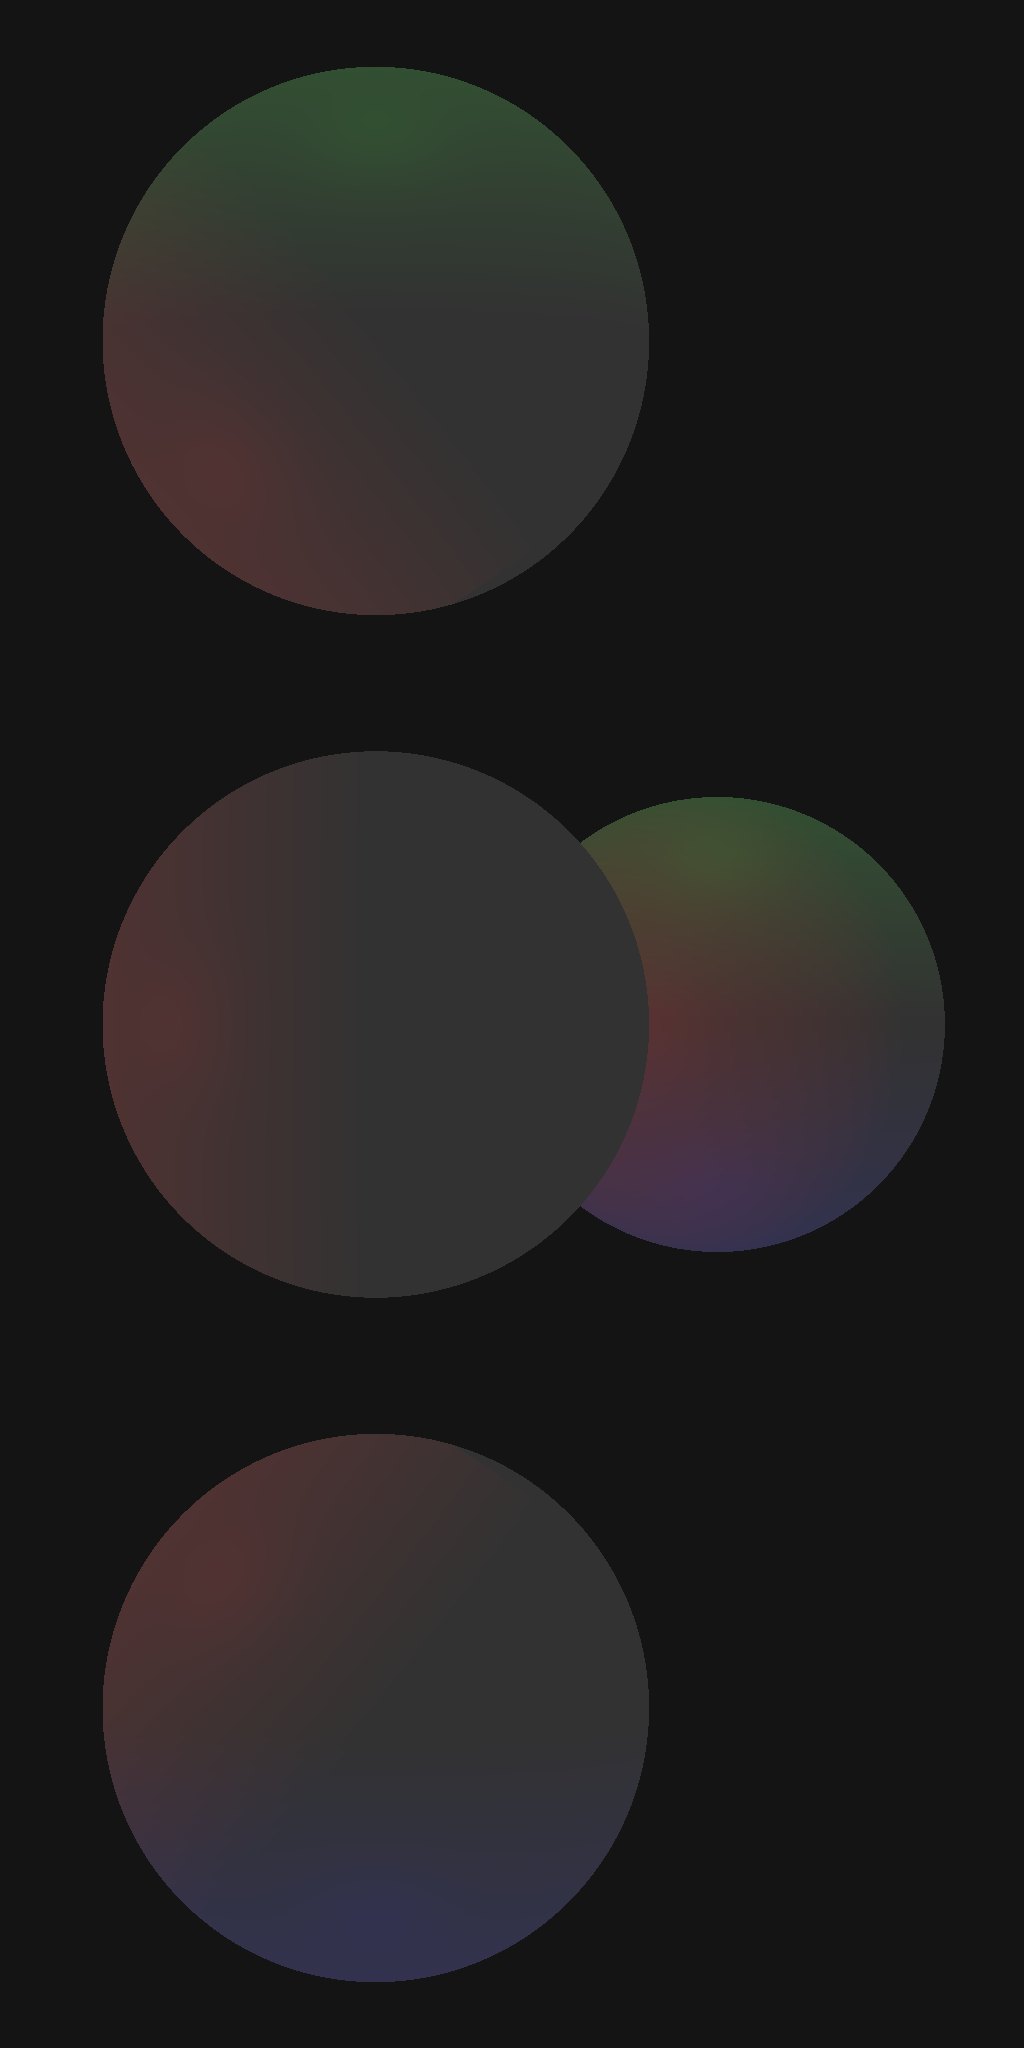
\includegraphics[width=3.5cm]{images/phong_global.png}
			\end{figure}
		\end{column}
		\begin{column}{3cm}
			\begin{figure}
				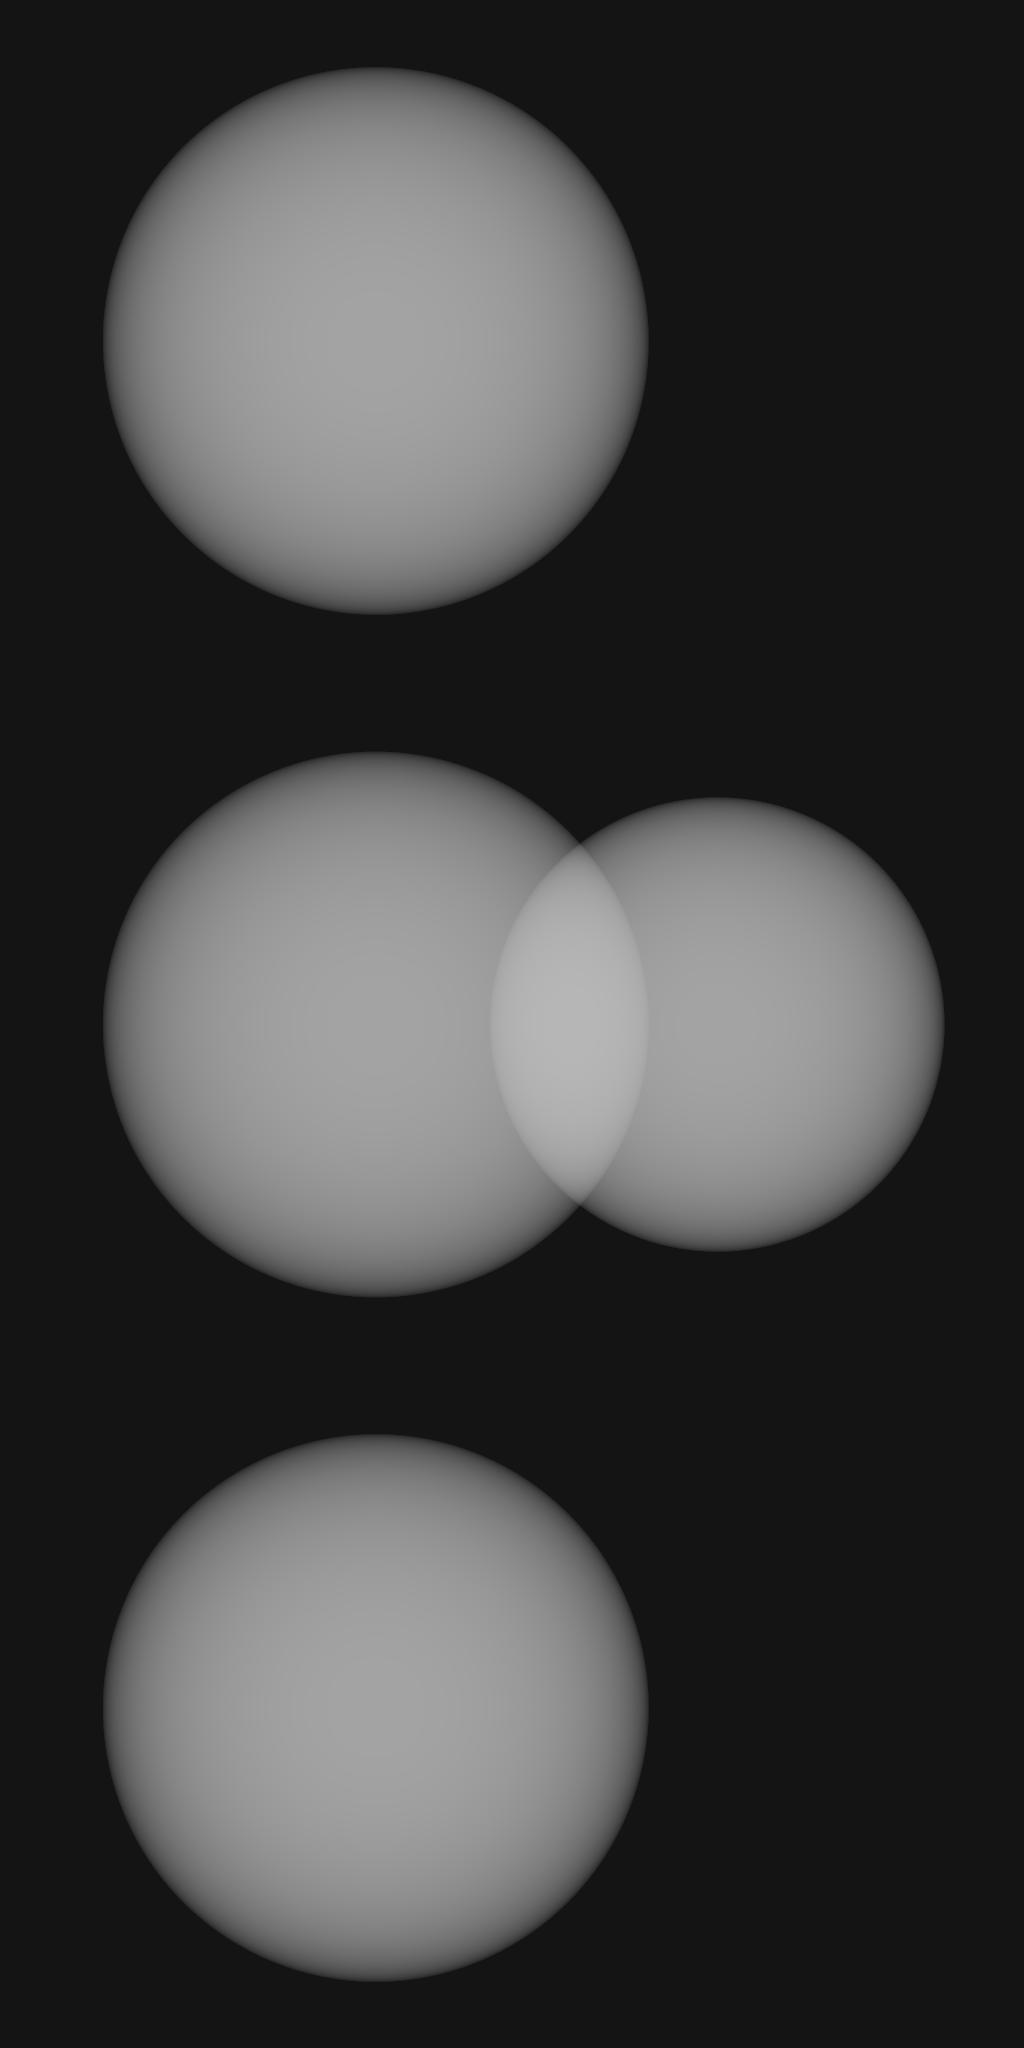
\includegraphics[width=3.5cm]{images/em_easy.png}
			\end{figure}
		\end{column}
		\begin{column}{3cm}
			\begin{figure}
				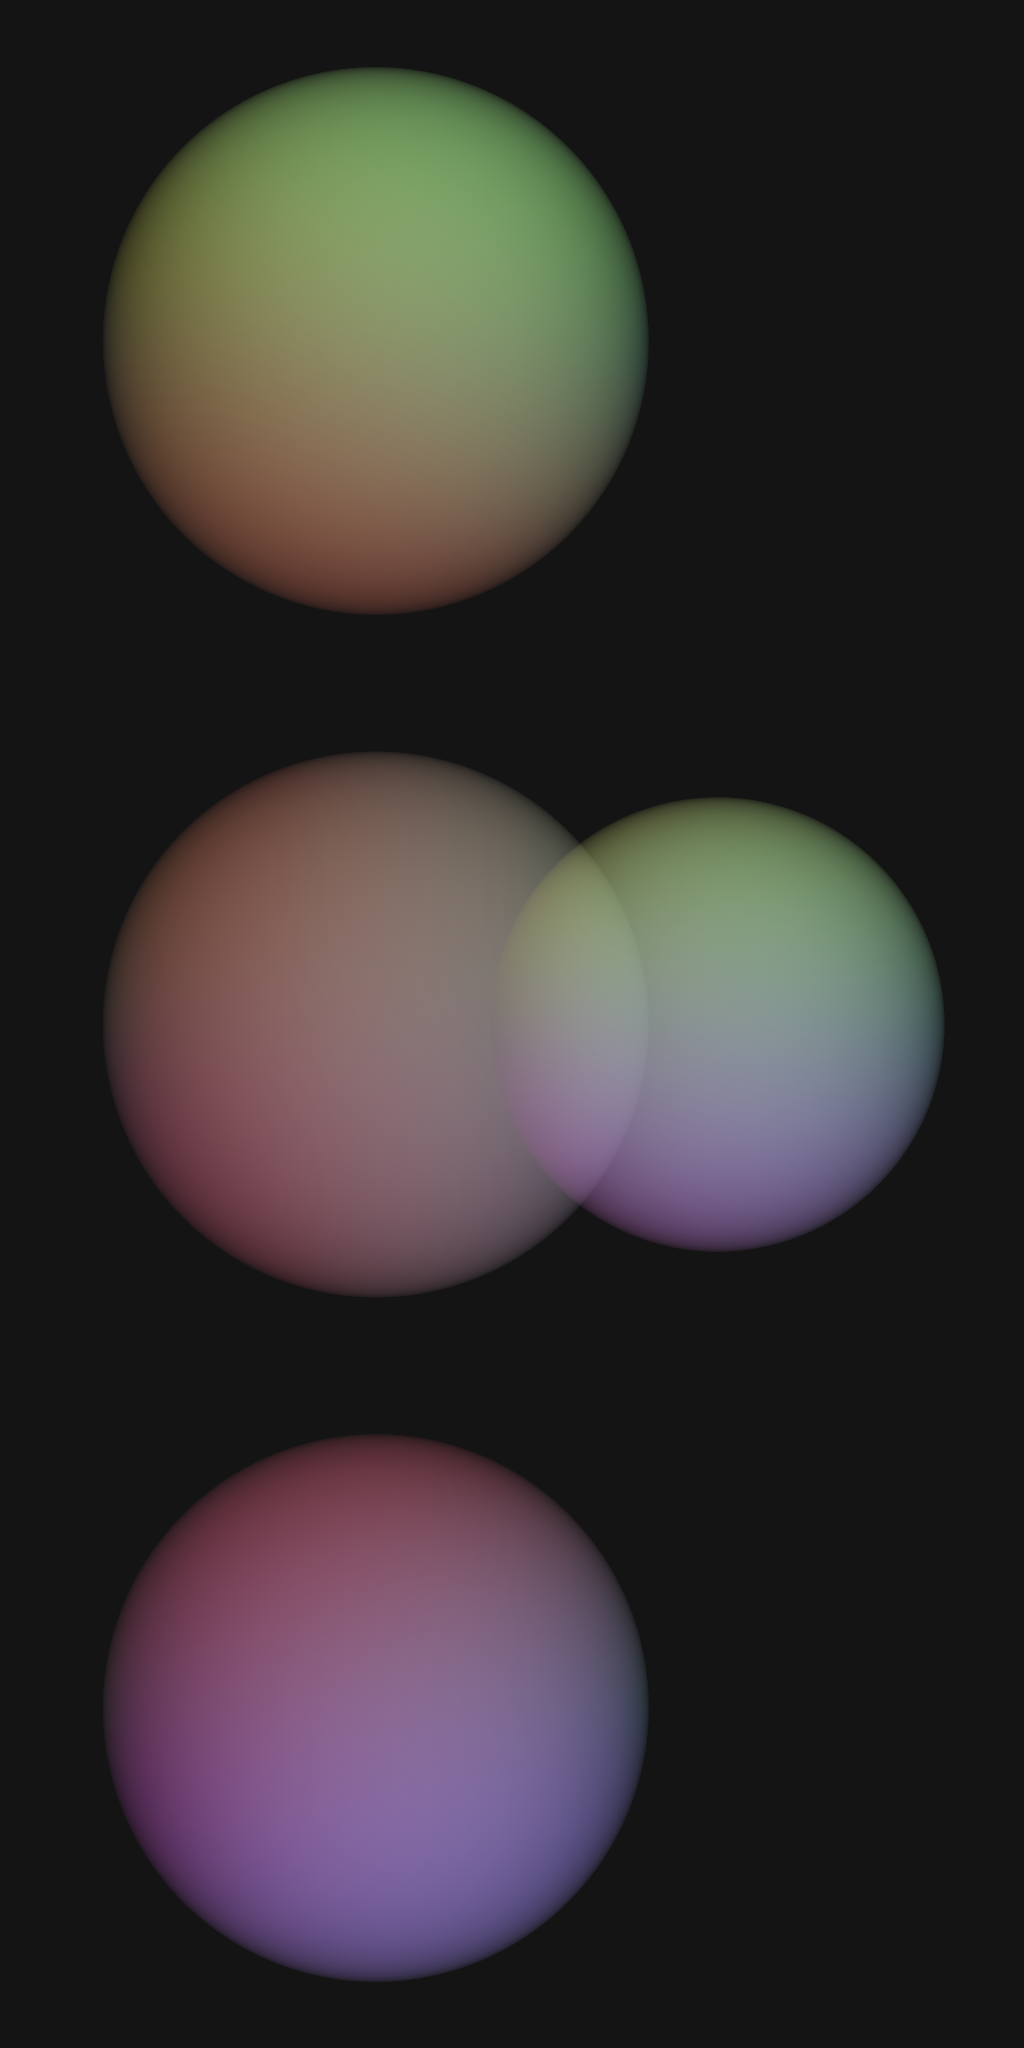
\includegraphics[width=3.5cm]{images/em_global.png}
			\end{figure}
		\end{column}
	\end{columns}
\end{frame}

\begin{frame}
	\frametitle{Wissenschaftliche Herausforderungen}
	
	Kugelglyphen werden mit Methoden der Volumendarstellung visualisiert: 
	
	\begin{itemize}
		\setlength{\itemsep}{8pt}
	
		\item physikalische Plausibilität des Modells
		\item weitestgehend Analytische Lösung
		\item kompakte und geschlossene Gleichung
		\item Genauigkeit wird Geschwindigkeit übergeordnet
		\item Ground-Truth
	\end{itemize}
	
	\vspace*{0.4cm}
	
	Unterstützte Effekte:
	
	\begin{itemize}
		\item Transparenz
		\item globaler Schattenwurf
	\end{itemize}
\end{frame}

\section{\textbullet \hspace{0.2cm} Fragen und Diskussion}
\begin{frame}
	\frametitle{Fragen und Diskussion}
	
	\begin{columns}
		\begin{column}{3cm}
			\begin{figure}
				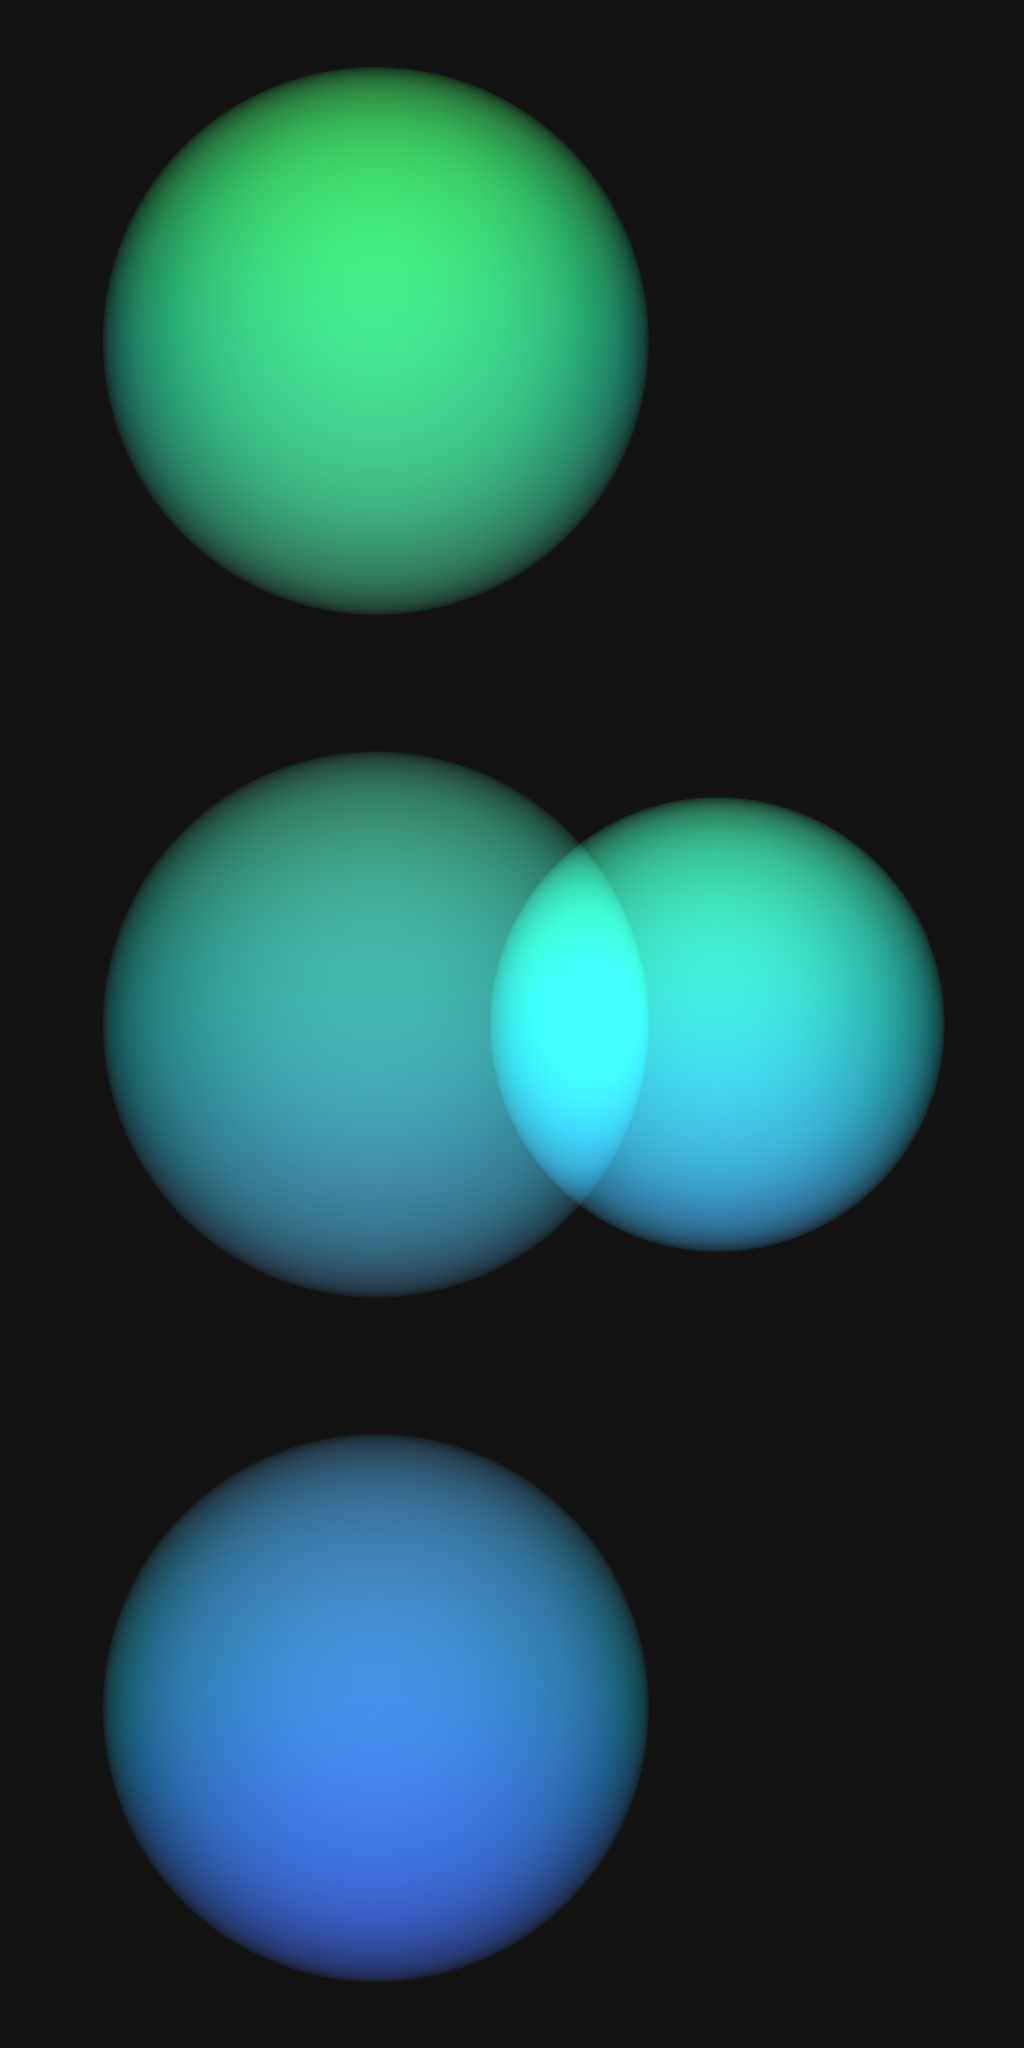
\includegraphics[width=3.5cm]{images/em_low.png}
			\end{figure}
		\end{column}
		\begin{column}{5cm}
			\begin{equation}
				\Theta(t_n, t_f) = 1 - \exp(- \lambda \textcolor{Purple}{\kappa} (t_f - t_n))
			\end{equation}
			
			\begin{equation}
				\kappa = - \frac{1}{\lambda \cdot 2r} \ln(1 - \Theta_{MAX})
			\end{equation}
		\end{column}
	\end{columns}

\end{frame}

{\tiny\bibliography{literatur}}

\end{document}
